
\documentclass[12pt]{article}
\usepackage{graphicx}
\usepackage{hyperref}

\begin{document}

\begin{center}
\textbf{ MAT 442: HMW 2}\\
\textbf{\ ERICAGYEMANG(Spring 2019)}\\
\end{center}

\textbf{1}. $y_{k+1} = -(1.1)y_k+0.1$ , $y_0=0$ where $a=-1.1,b=0.1$.\hspace{2cm}(1.0)\\
To find the solution to the above difference equation is appropriate is set up model that satisfies the relation $g(y)=(y)$.For easy computation, there is a need for a function with a detected pattern that will spit out sequence of solution $y_o,y_1,y_2,y_3,...$ of absolute real numbers.From (1.0) above we know that $a\ne1$ therefore we have to develop a model to arrive at our solution.Solving (1.0) by hand we detect a trend and pattern, substituting $y_o,y_1,y_2,y_3,....$ we get $0.1$,$-00.1$,$0.111$,...respectively.To clearly identify the pattern detected in the solution, we algebraically deduce the following : $y_1=ay_0+b$ , $y_2=a(ay_0+b)+b$ , $y_2=a(a^2y_0+ab+b)+b,...$ we can rewrite this sequence as
 \[y_k=a^ky_0+(a^{k-1}+...+a+1)b=a^ky_0+\frac{1-a^k}{1-a}b.\] Note that, since the question did not specify any biological significant assumption allowed to have negatives solutions and coefficients.




 \cleardoublepage        

 \textbf{2}. a. The Logistic model\\
 For figure 1 below, we started with our initial condition at 0.1 with up-right(clockwise movement),the dashed line with arrows clearly depicts the direction of the dashed arrow line moving around fixed point with coordinates(0.75,0.75) hence the behavior can be unpredictable causing the solutions not be attracted to the equilibrium point. 
\begin{figure} [ht!]
 \centering
 \includegraphics[height=2in]{/Users/ERICAGYEMANG/Desktop/Biomath/Figures/hw2.jpg} 
\caption[Figure 2.4: r>1]{Cobwebbing Method, $r=0.1$}
 \label{fig::model}
\end{figure}

 b.Ricker's model\\
 Figure 2, has a different fixed point where the curve intersects with line $z=y$.One interesting thing is that, we can see our dashed arrow line moving towards the fixed point with coordinates(1.3,1.3) and actually staying there because the fixed point absorbs our movement overtime.
\begin{figure} [ht!]
 \centering
 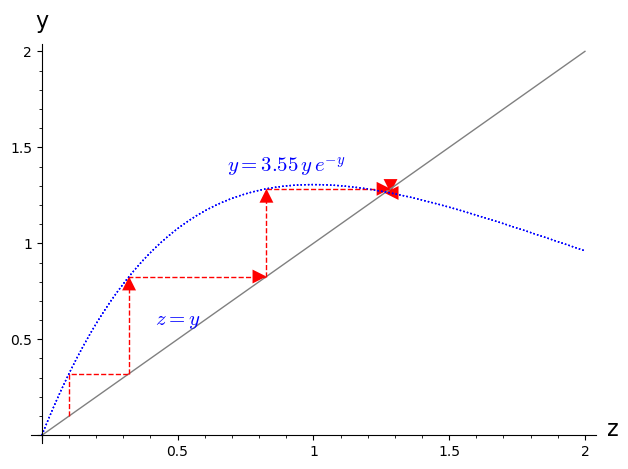
\includegraphics[height=2in]{/Users/ERICAGYEMANG/Desktop/Biomath/Figures/hww2.jpg} 
\caption[Figure 2.4: r>1]{Cobwebbing Method, $r=0.1$}
 \label{fig::model}
\end{figure}
 
 
 
 
 
  \cleardoublepage     
 
  \textbf{3}.\textbf{a} .\[y_{k+1}= \frac{1}{2}y_k +y^2_k-\frac{7}{144}\]\\
  Using the quadratic formula;$y=\frac{-b\pm\sqrt{b^2-4ac}}{2a}$ to derive the solutions for the difference equation, we set our notations to be $a=1/2,b=1,c=-7/144$ which gives us these solutions  $y_\infty^1=1/12$ and $y_\infty^1=-7/12$ to be our equilibrium points..In this exercise we considering just the positive equilibrium meaning we use  $y_\infty^1=1/12$.To determine whether equillibrium is asymptotically stable or not, we need to algebraically deduce it from $\left|f'(y_\infty^1)\right|$ where we set :
\[f(y)= \frac{1}{2}y +y^2-\frac{7}{144},\] 
\[f'(y)= 2y+0.5,\] 
 \[\left|f'(y_\infty^1)\right|= \left|f'(1/2)\right|=\left|2(1/2)+1/2\right|=\frac{2}{3},\]\\therefore $\left|f'(y_\infty^1)\right| < 1$,implies $y_\infty^1$ is LAS by definiton of equilibrium theorem.\vspace{1.0cm}

\textbf{b}. \[y_{k+1}=ry_k(1-y_k)\]
Finding the equilibrium of the logistic equation;
\[y_{k+1}=ry_k(1-y_k)=ry-ry^2,\]\\
where the recursion function is f(y)=ry(1-y).We solve the equation algebraically and derive two fixed points
 \[y_\infty^1=0\hspace{0.5cm} and\hspace{0.5cm} y_\infty^2=(1-1/r),\]where $r>1$.\\
 Now,the derivative of $f$ is\\
 \[f'(y)=ry-ry^2=r-2yr,\]we consider $y_\infty^2=(1-1/r)$ since the question expect us to use just the positive equilibria so
\[\left|f'(y_\infty^2)\right|=\left|f'(1-1/r)\right|=\left|r-2(1-r)r\right|=\left|2-r\right|,\]
analyzing the equilibrium point whether LAS or not,we perform some algebraic analysis such that
$(y_\infty^2)=(1-1/r)$ is LAS If $2-1<r<2+1\iff1<r<3$ and unstable if $0<r<3$ or $r>3$.\vspace{1.0cm}

 
  


  
\textbf{c}.\[y_{k+1}=\frac{ry^2_k}{y^2_k+A}\]
Using the quadratic formula;$y=\frac{-b\pm\sqrt{b^2-4ac}}{2a}$ to derive the solutions for the difference equation, we set our notations to be $a=1,b=-r,c=A,B=\sqrt{r^2-4A}$ such that,\[y=\frac{-r\pm\sqrt{r^2-4A}}{2}\Rightarrow y_+=\frac{r+B}{2}\hspace{0.1cm} or\hspace{0.1cm} y_-=\frac{r-B}{2}.\]
Now, we find the derivative of $f$ with respect to y and substitute our equilibrium points\\
\[f'(y)=ry^2(y^2+A)^{-1}=2ry(y^2+A)^{-1}-ry^2(y^2+A)^22y=2y\frac{rA}{(y^2+A)^2},\] 
\[f'(y_+)=\frac{4A}{r(r+B)}>0,f'(y_-)=\frac{4A}{r(r-B)}>0.\] since both derivatives are positive we make further analysis to show the first derivative is less 1 and second derivative is greater based on the parameters r and A.$f'(y_+)=\frac{4A}{r(r+B)}<1$ and $f'(y_-)=\frac{4A}{r(r-B)}>1$  if $r>2,A=1$.From the equilibrium stability theorem we understand $y_+$ is LAS and  $y_-$is unstable as long as they both exist.Referring back to the cobweb diagrams displayed in our textbook(page 36),the cobweb diagram depicts the solutions and graphically shows the behavior of the solutions which is identical to analysis made above algebraically.\vspace{1.0cm}

\cleardoublepage        

 
 




\begin{thebibliography}{99}
\bibitem{r1}http://dl.lateralis.org/public/sagebook/sagebook-ba6596d.pdf

\bibitem{r2}http://www.maths.usyd.edu.au/u/billg/MATH2052/tutorials/tutorial3/node8.html

\end{thebibliography}

\end{document}